
\setcounter{chapter}{1}
\chapter{Business Understanding and Comparative
Analysis}
\minitoc %insert la minitoc
\graphicspath{{Chapitre2/figures/}}

%\DoPToC

%==============================================================================
\pagestyle{fancy}
\fancyhf{}
\fancyhead[R]{\bfseries\rightmark}
\fancyfoot[R]{\thepage}
\renewcommand{\headrulewidth}{0.5pt}
\renewcommand{\footrulewidth}{0pt}
\renewcommand{\chaptermark}[1]{\markboth{\MakeUppercase{\chaptername~\thechapter. #1 }}{}}
\renewcommand{\sectionmark}[1]{\markright{\thechapter.\thesection~ #1}}

\begin{spacing}{1.2}
%==============================================================================

\section*{Introduction}
This chapter establishes the theoretical and contextual foundation of the project. It begins with an overview of the software development lifecycle (SDLC) and the role of emerging AI technologies such as Large Language Models (LLMs), Generative AI, and AI agents in modern software engineering. It then presents the state of the art by reviewing existing solutions currently supporting code quality and best practices. Finally, it defines the project requirements, both functional and non-functional, showing how this work addresses existing gaps by integrating AI-driven assistance into a key phase of the SDLC.  

\section{Business and Reasoning}

\subsection{Software Development Life Cycle (SDLC)}

The Software Development Life Cycle (SDLC) is a structured framework that defines the process of planning, creating, testing, deploying, and maintaining software systems. It ensures that software development follows a disciplined approach, promoting quality, efficiency, and maintainability while reducing risks and development costs. The SDLC helps teams manage complex projects by providing a roadmap from initial requirements to system retirement.  

\begin{figure}[H]
    \centering
    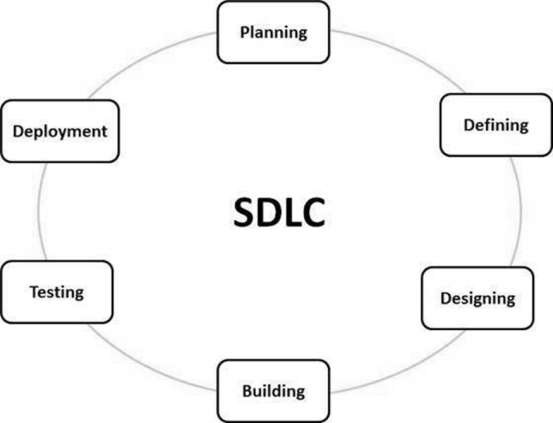
\includegraphics[scale=0.65]{Images/sdlc_stages.jpg}
    \caption{Software Development Life Cycle Overview}
    \label{fig:sdlc_cycle}
\end{figure}

\subsubsection*{Key Steps in SDLC}
A typical SDLC consists of seven core phases, each serving a distinct purpose in ensuring that software meets functional and quality requirements:

\begin{enumerate}
    \item \textbf{Planning:} This initial phase defines the project scope, objectives, resources, and timeline. Risk assessment, feasibility studies, and cost-benefit analyses are performed to ensure the project is viable before investing substantial resources.
    
    \item \textbf{Requirements Analysis:} Stakeholders, including end-users and business analysts, collaborate to specify functional and non-functional requirements. Clear, documented requirements reduce ambiguity and serve as a reference for design and implementation. Techniques such as use cases, user stories, and requirement specifications are commonly used.
    
    \item \textbf{System Design:} Architects and developers define the software architecture, data models, interface designs, and technology stack. This phase produces detailed design documents and prototypes that guide the implementation phase.
    
    \item \textbf{Implementation (Coding):} Developers translate design specifications into source code using appropriate programming languages, frameworks, and tools. Best practices such as modularization, code reviews, and version control are critical in this phase.
    
    \item \textbf{Testing:} The system undergoes rigorous verification to detect and correct defects. Testing can include unit testing, integration testing, system testing, performance testing, and user acceptance testing (UAT). Automated testing frameworks are increasingly used to ensure efficiency and repeatability.
    
    \item \textbf{Deployment:} Once verified, the software is deployed to production environments. Deployment strategies may include phased rollouts, blue-green deployments, or canary releases to minimize risk and disruption.
    
    \item \textbf{Maintenance:} After deployment, the software requires ongoing updates, bug fixes, performance improvements, and adaptations to changing requirements or environments. Maintenance ensures long-term system reliability and user satisfaction.
\end{enumerate}

\subsubsection*{Common SDLC Models}
Various SDLC models provide different approaches to organizing these steps. Each model offers specific advantages and trade-offs, depending on project complexity, team structure, and business goals.

\paragraph{Waterfall Model}
The Waterfall model is a linear and sequential approach where each phase must be completed before the next begins. Its structure ensures strict documentation and clear progress milestones.  

\begin{figure}[H]
    \centering
    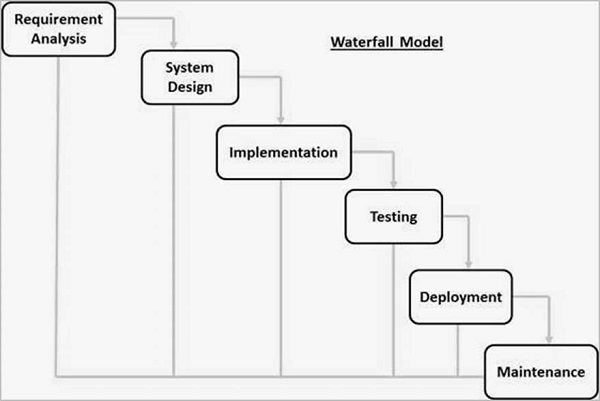
\includegraphics[scale=0.6]{Images/sdlc_waterfall_model.jpg}
    \caption{Waterfall SDLC Model}
    \label{fig:waterfall_model}
\end{figure}

\textbf{Advantages:} Simple and easy to manage, clear documentation, predictable timelines.\\ 
\textbf{Limitations:} Inflexible to changing requirements, late discovery of defects, high risk in complex projects.  

\paragraph{V-Model (Verification and Validation)}
The V-Model extends Waterfall by emphasizing verification and validation. Each development phase has a corresponding testing phase to ensure quality at every stage.  

\begin{figure}[H]
    \centering
    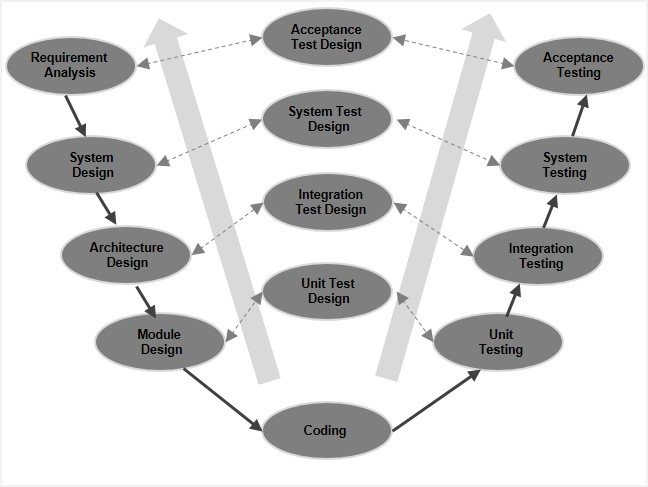
\includegraphics[scale=0.8]{Images/sdlc_v_model.jpg}
    \caption{V-Model SDLC}
    \label{fig:v_model}
\end{figure}

\textbf{Advantages:} Strong focus on testing, early defect detection.\\ 
\textbf{Limitations:} Like Waterfall, less flexible with changing requirements.  

\paragraph{Iterative and Incremental Model}
This approach develops software in small iterations, delivering functional increments at each cycle. Feedback from early releases informs subsequent iterations.  

\begin{figure}[H]
    \centering
    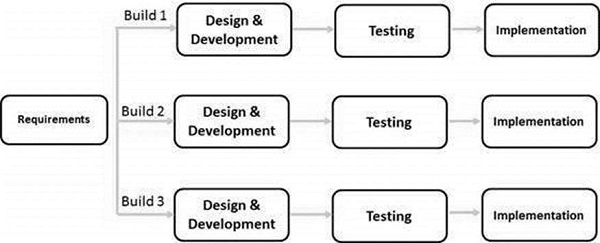
\includegraphics[scale=0.6]{Images/sdlc_iterative_model.jpg}
    \caption{Iterative and Incremental SDLC Model}
    \label{fig:iterative_model}
\end{figure}

\textbf{Advantages:} Flexibility to change, early delivery of usable software, reduced risk.\\  
\textbf{Limitations:} Requires careful planning, can increase complexity if iterations are poorly managed.  

\paragraph{Agile Model}
Agile emphasizes collaboration, adaptability, and rapid delivery. Work is organized into sprints, typically 2-4 weeks, producing a potentially shippable product increment. 
Agile can be implemented through frameworks such as:

\begin{itemize}
    \item \textbf{Scrum:} Defines roles (Product Owner, Scrum Master, Development Team) and ceremonies (Daily Stand-ups, Sprint Planning, Retrospectives) to organize work in sprints.
    \item \textbf{Kanban:} Visualizes workflow and limits work in progress, emphasizing continuous delivery and efficiency rather than fixed-length iterations.
\end{itemize}

\begin{figure}[H]
    \centering
    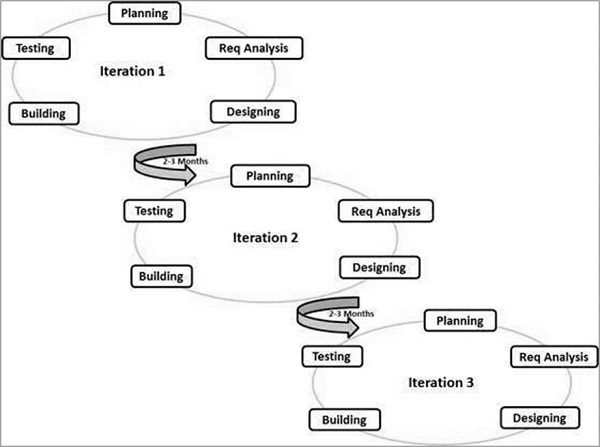
\includegraphics[scale=0.65]{Images/sdlc_agile_model.jpg}
    \caption{Agile SDLC Model}
    \label{fig:agile_model}
\end{figure}

\textbf{Advantages:} Highly flexible, promotes continuous feedback, encourages customer involvement.\\ 
\textbf{Limitations:} Less predictability in timelines, requires disciplined team practices.  


\paragraph{DevOps}
DevOps is a cultural and technical approach that integrates development and operations teams, promoting continuous integration, continuous delivery (CI/CD), automated testing, and real-time monitoring. By combining SDLC phases with DevOps practices, organizations achieve faster delivery, higher reliability, and improved collaboration between teams.

\begin{figure}[H]
    \centering
    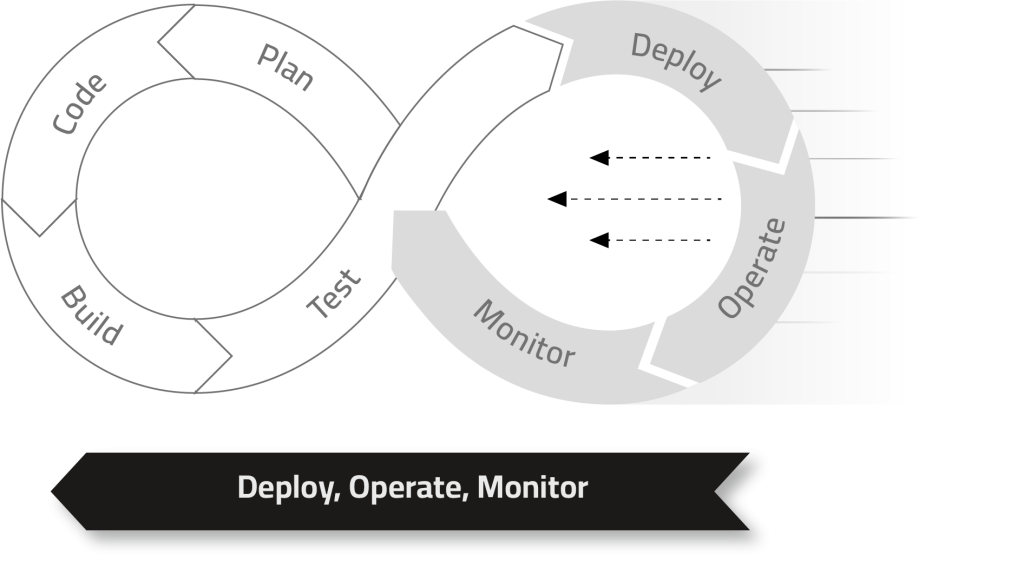
\includegraphics[scale=0.3]{Images/devops.png}
    \caption{DevOps Cycle Integration with SDLC}
    \label{fig:devops_cycle}
\end{figure}

\textbf{Advantages:} Accelerates delivery, improves collaboration, enables automated testing and monitoring, enhances reliability.\\
\textbf{Limitations:} Requires organizational culture change, relies on mature tooling, can be complex to implement in large teams.

\paragraph{Emerging Enhancements}
Modern software development also increasingly relies on AI-powered tools that provide predictive analytics, code suggestions, and real-time quality checks. These enhancements further increase SDLC efficiency and reliability, setting the stage for intelligent, AI-driven development assistance.



\subsection{Artificial Intelligence in Software Development}

%-------------------------
\subsubsection*{Foundational AI Concepts}
Artificial Intelligence (AI) refers to computational systems capable of performing tasks that typically require human intelligence, such as reasoning, learning, problem-solving, and decision-making. AI encompasses a broad spectrum of techniques and paradigms, each with distinct capabilities and applications.

\begin{figure}[H]
    \centering
    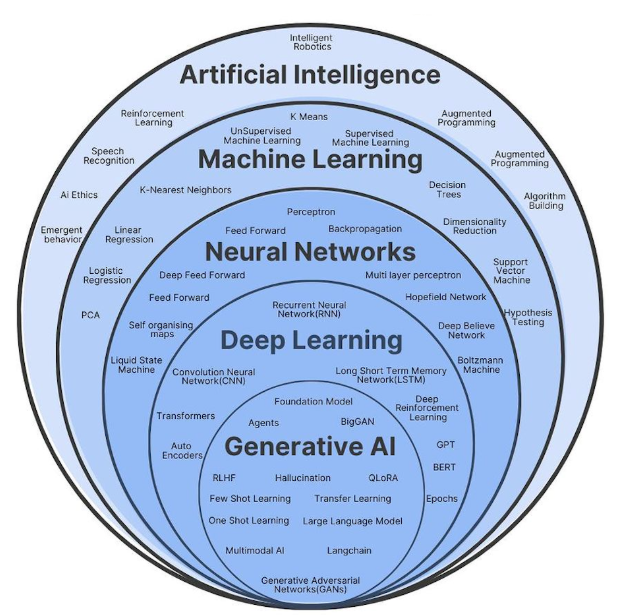
\includegraphics[scale=0.6]{Images/AI.png}
    \caption{Hierarchy of AI Technologies}
    \label{fig:ai_hierarchy}
\end{figure}

The AI landscape includes several key categories:

\begin{itemize}
    \item \textbf{Symbolic AI:} Systems based on rules and logic to represent knowledge and perform reasoning. These systems excel at tasks with well-defined rules but struggle with ambiguity and complex pattern recognition.
    
    \item \textbf{Machine Learning (ML):} Algorithms that improve performance on tasks by learning from data rather than being explicitly programmed. ML systems can identify patterns and make predictions based on historical data.
    
    \item \textbf{Deep Learning (DL):} A subset of ML using artificial neural networks with multiple layers to model complex patterns in data. Deep learning has revolutionized fields like computer vision and natural language processing.
    
    \item \textbf{Generative AI:} AI systems capable of producing new content, such as text, code, or images, by learning patterns from existing datasets. Unlike traditional AI that classifies or predicts, generative AI creates novel outputs.
\end{itemize}

\subsubsection*{The AI Revolution in Software Engineering}
As software development becomes increasingly complex and teams face mounting pressure to deliver high-quality code faster, traditional development approaches are reaching their limits. The emergence of Artificial Intelligence technologies presents a transformative opportunity to address these challenges by bringing intelligent assistance directly into the development workflow.

The integration of AI into software development represents more than just technological advancement—it addresses fundamental business challenges that organizations face in maintaining code quality, reducing technical debt, and scaling development practices across growing teams. This represents a paradigm shift from traditional SDLC approaches to what we can call the AI-Enhanced SDLC—a development lifecycle where intelligent assistance is embedded throughout every phase, creating a more efficient, proactive, and intelligent development process.

This transformation is primarily driven by two key AI technologies: Large Language Models (LLMs) and AI agents, which together enable the intelligent development workflows that characterize the modern AI-enhanced SDLC.

\subsubsection*{Large Language Models: The Foundation of Intelligent Development}
Large Language Models (LLMs) represent a breakthrough in generative AI technology, trained on massive corpora of natural language and source code. Unlike traditional programming tools that rely on rigid rules and patterns, LLMs understand context, semantics, and intent, making them uniquely suited for complex reasoning tasks across various domains.

\begin{figure}[H]
    \centering
    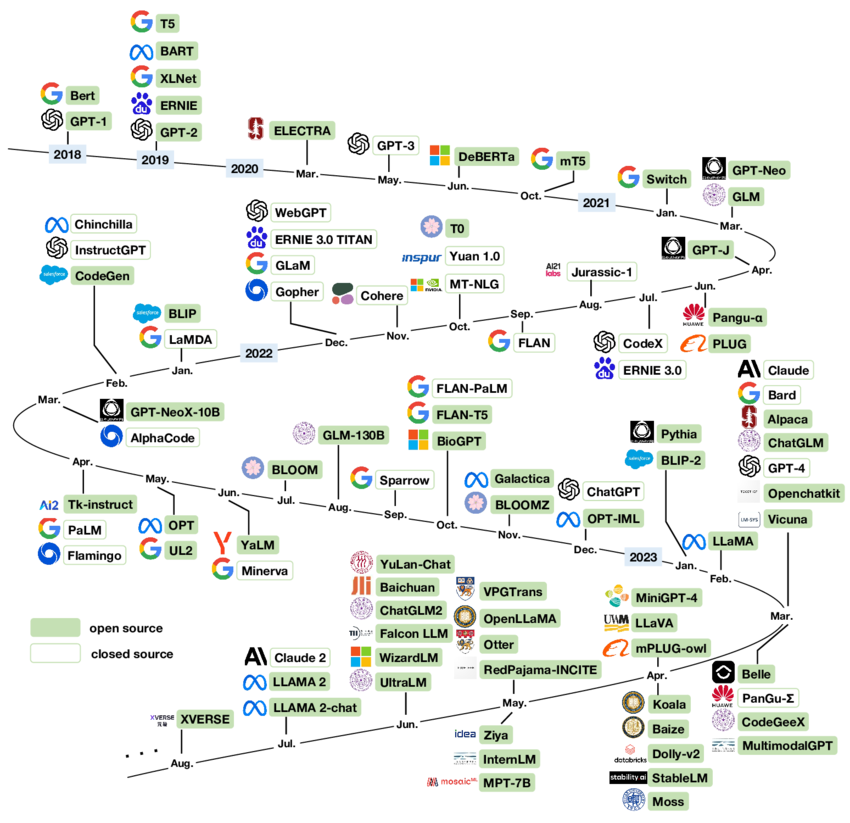
\includegraphics[scale=1]{Images/A-chronological-overview-of-large-language-models-LLMs-multimodal-and-scientific.png}
    \caption{A chronological overview of large language models (LLMs) [2018-2024]}
    \label{fig:llm_overview}
\end{figure}

The fundamental capabilities of LLMs include:

\begin{itemize}
    \item \textbf{Natural Language Understanding:} Ability to comprehend and interpret human language with nuanced understanding of context, intent, and meaning.
    \item \textbf{Pattern Recognition:} Capacity to identify complex patterns in data, including code structures, design patterns, and domain-specific conventions.
    \item \textbf{Content Generation:} Capability to produce coherent, contextually appropriate text, code, and other content based on learned patterns.
    \item \textbf{Reasoning and Inference:} Ability to perform logical reasoning, make inferences, and solve complex problems through step-by-step analysis.
\end{itemize}

In the context of software development, these capabilities translate into powerful applications:

\begin{itemize}
    \item \textbf{Contextual Code Analysis:} Understanding code within its broader project context, including relationships between components, dependencies, and business logic.
    \item \textbf{Intelligent Code Generation:} Producing code suggestions, refactoring recommendations, and automated fixes that align with project-specific patterns and requirements.
    \item \textbf{Explanatory Documentation:} Providing clear, human-readable explanations of code behavior, potential issues, and suggested improvements.
    \item \textbf{Semantic Standards Enforcement:} Detecting violations of coding standards and best practices that go beyond simple syntax checking to include design patterns, architectural principles, and domain-specific guidelines.
\end{itemize}

\subsubsection*{AI Agents: Orchestrating Intelligent Development Workflows}

While LLMs provide the foundational intelligence for understanding and generating code, AI agents represent the next evolution—autonomous systems that can reason, plan, and execute complex development tasks. AI agents serve as intelligent orchestrators that bridge the gap between human developers and AI capabilities, providing seamless integration of AI assistance into the development workflow.

\paragraph{Agent Architecture and Workflow}

The architecture of AI agents follows a structured workflow that enables reliable and scalable operation. As illustrated in Figure \ref{fig:ai_agent_workflow}, the agent orchestration process begins with input processing, where user requests are captured and preprocessed. The core reasoning component then analyzes the input using LLM capabilities to determine the appropriate course of action. This is followed by tool integration, where the agent interfaces with external systems to execute planned actions. Throughout this process, the memory layer maintains context and stores relevant information for future reference.

\begin{figure}[H]
    \centering
    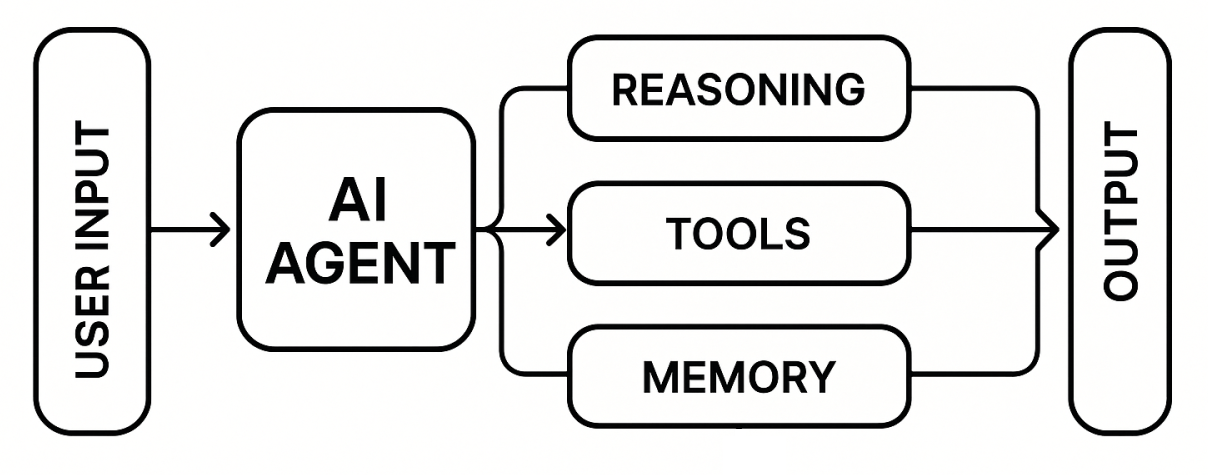
\includegraphics[scale=0.2]{Images/ai_agent.png}
    \caption{AI Agent Architecture and Orchestration Workflow}
    \label{fig:ai_agent_workflow}
\end{figure}

\paragraph{Core Components of Development-Focused AI Agents}

AI agents designed for software development incorporate specialized components tailored to the development workflow:

\begin{itemize}
    \item \textbf{Code Analysis Engine:} Processes source code, understands project context, and identifies violations of coding standards, design patterns, and best practices.
    
    \item \textbf{Contextual Reasoning:} Utilizes LLMs to understand the broader project context, including dependencies, business logic, and architectural constraints when making recommendations.
    
    \item \textbf{Development Tool Integration:} Interfaces with IDEs, version control systems, testing frameworks, and other development tools to provide seamless assistance within the existing workflow.
    
    \item \textbf{Learning and Adaptation:} Continuously learns from codebase patterns, team feedback, and project outcomes to provide increasingly relevant and accurate assistance.
    
    \item \textbf{Feedback and Explanation System:} Provides clear, actionable explanations for identified issues and suggested improvements, helping developers understand not just what to change, but why.
\end{itemize}


\paragraph{Balancing AI Capabilities with Practical Considerations}

While AI agents offer transformative potential for software development, their deployment requires careful consideration of both capabilities and limitations:

\textbf{Key Capabilities:}
\begin{itemize}
    \item \textbf{Contextual Understanding:} Ability to analyze code within its broader project context, understanding relationships and dependencies
    \item \textbf{Automated Analysis:} Consistent, comprehensive code analysis that scales across large codebases and development teams
    \item \textbf{Intelligent Recommendations:} Context-aware suggestions that go beyond simple rule-based checks to include design patterns and architectural considerations
    \item \textbf{Continuous Learning:} Adaptation to project-specific patterns and team preferences over time
\end{itemize}

\textbf{Practical Limitations:}
\begin{itemize}
    \item \textbf{Computational Cost:} LLM-based analysis requires significant computational resources, impacting response times and operational costs
    \item \textbf{Context Constraints:} Limited ability to process extremely large files or maintain context across very long code sequences
    \item \textbf{Accuracy Considerations:} Potential for misinterpretation or hallucination, requiring human oversight for critical decisions
    \item \textbf{Integration Complexity:} Requires careful integration with existing development tools and workflows
\end{itemize}

These considerations inform the design of practical AI-assisted development systems that maximize benefits while managing limitations effectively.

\subsubsection*{AI-Enhanced SDLC: The Complete Integration}

The combination of LLMs and AI agents enables the complete integration of intelligent assistance throughout the software development lifecycle. This AI-enhanced SDLC represents a fundamental transformation from traditional reactive approaches to proactive, intelligent development assistance that addresses the core business challenges identified earlier.

\paragraph{The Transformative Impact of AI Integration}

The integration of AI into the SDLC addresses key limitations of conventional development practices:

\begin{itemize}
    \item \textbf{From Reactive to Proactive:} Traditional approaches identify issues after they occur, often during code review or testing phases. AI-enhanced development provides real-time feedback during coding, preventing issues before they become embedded in the codebase.
    
    \item \textbf{From Inconsistent to Scalable:} Human-based quality assurance varies in consistency and availability. AI provides uniform, expert-level analysis that scales across teams and projects without degradation.
    
    \item \textbf{From Static to Adaptive:} Traditional tools rely on fixed rules and patterns. AI systems learn and adapt to project-specific patterns, team preferences, and evolving best practices.
    
    \item \textbf{From Isolated to Integrated:} Rather than treating quality assurance as a separate phase, AI integrates intelligent assistance throughout the entire development workflow.
\end{itemize}

\paragraph{AI Applications Across the Development Lifecycle}

AI technologies provide targeted assistance at each phase of the SDLC, addressing specific challenges and opportunities:

\begin{itemize}
    \item \textbf{Requirements and Planning:} AI analyzes historical project data to predict timelines, identify requirement ambiguities, and suggest optimal resource allocation. Natural language processing helps translate business requirements into technical specifications.
    
    \item \textbf{Design and Architecture:} AI assists architects by analyzing existing codebases, suggesting architectural patterns, detecting design anti-patterns, and ensuring consistency with organizational standards.
    
    \item \textbf{Implementation:} This is where AI agents provide the most immediate value, offering real-time code completion, best practice enforcement, bug detection, and refactoring suggestions directly within the development environment.
    
    \item \textbf{Testing and Quality Assurance:} AI generates comprehensive test cases, prioritizes test execution based on risk analysis, and identifies edge cases that human testers might miss.
    
    \item \textbf{Deployment and Maintenance:} AI monitors deployment health, predicts potential issues, and automatically suggests optimizations based on usage patterns and performance metrics.
\end{itemize}

This comprehensive understanding of AI's potential in software development provides the foundation for evaluating current solutions and identifying opportunities for improvement. The next section examines existing approaches to code quality and best practices enforcement, highlighting both their contributions and limitations in addressing the business challenges outlined above.

\section{State of the Art: Existing Solutions}

While the AI-enhanced SDLC presents a vision of intelligent, proactive development assistance, the current reality in most development environments, including our workspace, relies on more traditional approaches to code quality and best practices enforcement. Software engineers currently depend on a combination of human review, automated scripts, and rule-based systems to maintain code quality. These mechanisms vary in scope, effectiveness, and feedback timing, but as our analysis will show, they leave significant gaps in providing the real-time, intelligent assistance that characterizes the AI-enhanced development paradigm.

\paragraph{Current Feedback Mechanisms}
The existing approaches to code quality and best practices enforcement can be categorized into several key mechanisms:

\begin{itemize}
    \item \textbf{Code Reviews:} Human reviewers examine code for design quality, readability, maintainability, and adherence to standards. While this approach provides high-level, context-aware feedback, it often introduces delays and requires significant effort. Recently, AI-assisted review tools have been developed to accelerate this process by providing initial suggestions or flagging common issues.
    
    \item \textbf{Presubmit Checks:} Automated scripts that validate code before submission, enforcing style guides, ensuring compilation, and verifying simple correctness and safety constraints. Although fast and reliable, they primarily focus on surface-level checks and do not consider design or contextual issues.
    
    \item \textbf{Rule-Based Checks:} Systems that enforce coding conventions, naming schemes, and formatting standards. These tools provide consistency and objectivity but cannot reason about complex or context-dependent best practices.
    
\end{itemize}

\paragraph{Limitations}
While valuable, these approaches leave significant gaps, particularly in providing timely and intelligent feedback during the active coding phase. This timeline illustrates where current feedback mechanisms fit into the developer workflow:

\begin{figure}[H]
    \centering
    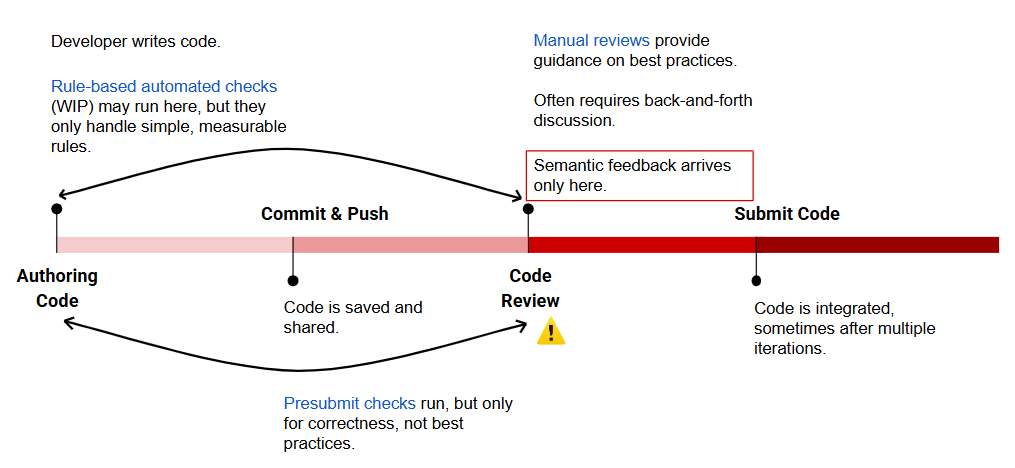
\includegraphics[scale=0.9]{Images/developer_workflow_feedback_timeline.png}
    \caption{Current Developer Workflow Feedback Timeline}
    \label{fig:developer_workflow_feedback_timeline}
\end{figure}

During the \textbf{Coding Phase}, developers get some support from Rule-Based Checks, but these are limited to simple, objective rules and often miss the nuances of complex best practices. 

The most insightful feedback on design and best practices typically comes during \textbf{Code Review}, but this happens after the initial development, making changes more disruptive.

Finally, \textbf{Presubmit Checks} before submission focus on correctness and safety, not on proactive best practice guidance.

This leaves a significant gap: there's no real-time, intelligent support for adhering to complex best practices while the developer is actively coding, which is the gap our project aims to fill.

\begin{table}[H]
\centering
\begin{tabular}{|p{4cm}|p{5cm}|p{5cm}|}
\hline
\textbf{Approach} & \textbf{Strengths} & \textbf{Limitations} \\
\hline
Code Reviews & Context-aware, high-level insights & Feedback delayed, time-consuming \\
\hline
Presubmit Checks & Fast, automated validation & Limited scope, mostly syntax and safety \\
\hline
Rule-Based Checks & Consistency, objectivity & Cannot handle complex or contextual practices \\
\hline
\end{tabular}
    \caption{Comparison of available software quality support solutions}
\label{tab:extended_solutions}
\end{table}

    
\paragraph{Impact of Delayed Feedback}
Following from the previous analysis, these workflow issues create concrete impacts on development:

\begin{itemize}
    \item \textbf{Technical Debt Accumulation:} Delayed feedback and limited enforcement of best practices lead to accumulating technical debt and inconsistencies in code quality over time.
    
    \item \textbf{Prolonged Review Cycles:} Review cycles take longer because developers must iterate multiple times to address issues discovered late in the process.
    
    \item \textbf{Developer Frustration:} The repetitive cycle of late-stage corrections contributes to developer frustration and reduced productivity.
    
    \item \textbf{Inconsistent Quality Standards:} Without real-time guidance, adherence to best practices varies significantly across team members and projects.
    
    \item \textbf{Increased Development Costs:} The cost of fixing issues increases exponentially the later they are discovered in the development process.
\end{itemize}

This analysis clearly demonstrates why we need a solution that brings guidance earlier, directly into the authoring process, addressing the fundamental timing and intelligence gaps in current approaches.




\paragraph{Trends and Emerging Practices}
Modern development increasingly integrates AI-driven assistance, predictive code analysis, automated documentation, and intelligent testing recommendations. These trends aim to provide proactive, context-aware guidance within the IDE, reducing errors and improving developer efficiency. However, as our analysis shows, there remains a critical gap in providing real-time, intelligent feedback during the active coding phase.

The limitations identified in current approaches—delayed feedback, limited scope of automated checks, and inability to handle complex best practices—create a compelling case for integrating LLM-powered assistance directly into the development workflow. This represents the next evolution in development tooling, moving from reactive quality assurance to proactive, intelligent guidance that addresses the fundamental gaps in current solutions.

---

\section{Project Requirements}

To tackle the issue of delayed feedback and limited intelligent assistance, our solution integrates the power of large language models directly into the developer's workflow in the IDE.

The proposed system builds on gaps identified in existing solutions. It aims to provide real-time, AI-driven feedback directly in the developer workflow, while maintaining performance, scalability, and usability.

\subsection{Functional Requirements}
The system must:
\begin{itemize}
    \item \textbf{Detect Framework Violations:} Identify violations of internal YouTube framework best practices and coding standards in real-time during development.
    
    \item \textbf{Provide Contextual Explanations:} Explain violations in clear, developer-friendly language with context-specific rationale that helps developers understand why certain patterns are problematic.
    
    \item \textbf{Generate Actionable Fixes:} Suggest specific, actionable fixes leveraging AI-generated solutions tailored to YouTube framework patterns and conventions.
    
    \item \textbf{Enable Developer Interaction:} Allow developers to accept, reject, or modify AI suggestions, providing full control over the implementation of recommended changes.
    
    \item \textbf{Maintain Contextual Relevance:} Ensure feedback appears in the appropriate location within the code and remains relevant and accurate as the developer continues coding.
    
    \item \textbf{Seamless IDE Integration:} Integrate seamlessly with the existing internal IDE, extension, and backend workflow without disrupting the developer's current development process.
\end{itemize}

\subsection{Non-Functional Requirements}
The system should also meet broader quality criteria:
\begin{itemize}
    \item \textbf{Performance:} Provide fast, near real-time responses to avoid interrupting developer workflow.
    \item \textbf{Scalability:} Efficiently handle large codebases and multiple simultaneous users.
    \item \textbf{Maintainability:} Enable modular updates, addition of new AI models, or coding rules.
    \item \textbf{Reliability:} Ensure robustness in production environments with minimal downtime.
    \item \textbf{Security and Privacy:} Comply with organizational policies, ensuring safe handling of code and data.
    \item \textbf{Usability:} Deliver concise, context-aware, and minimally intrusive feedback.
    \item \textbf{Extensibility:} Easily add new rules, models, or integrations.
\end{itemize}

\begin{table}[H]
\centering
\begin{tabular}{|p{6cm}|p{8cm}|}
\hline
\textbf{Requirement Type} & \textbf{Description} \\
\hline
Functional & Framework violation detection, contextual explanations, actionable fixes, developer interaction, contextual relevance, seamless IDE integration \\
\hline
Non-Functional & Performance, scalability, maintainability, reliability, security, usability, extensibility \\
\hline
\end{tabular}
\caption{Summary of project requirements}
\label{tab:extended_requirements}
\end{table}

\paragraph{Rationale}
These requirements address limitations identified in existing solutions by embedding proactive, context-aware feedback directly in the coding workflow, specifically targeting YouTube framework best practices. This approach enhances developer productivity, reduces framework-specific errors, and supports consistent adherence to internal YouTube development standards.


\section*{Conclusion}
This chapter established the business and theoretical foundation for integrating AI into software development workflows. Beginning with an analysis of the Software Development Life Cycle, it identified key challenges in maintaining code quality and consistency across growing development teams. The exploration of AI technologies—particularly Large Language Models and AI agents—revealed their potential for addressing these challenges through proactive, context-aware assistance.

The examination of existing solutions highlighted significant limitations: traditional tools provide limited analysis, and human review offers inconsistent feedback. There remains a critical gap in delivering real-time, intelligent assistance that scales with team growth. The AI-enhanced SDLC paradigm addresses these limitations by embedding intelligent assistance throughout the development process.

The project requirements defined in this chapter focus on real-time, AI-driven feedback for YouTube framework best practices that integrates seamlessly into the development workflow. The proposed solution bridges the gap between AI potential and practical development needs, setting the stage for the detailed system design presented in the following chapter.  








%==============================================================================
\end{spacing}


